\chapter{Sequenzdiagramme}
Die folgenden Sequenzdiagramme sollen den Ablauf von einzelnen Anwendungsfällen im PaVoS-System illustrieren. Die Interaktionen der Klassen miteinander in verschiedenen Situationen wird somit verdeutlicht.

\section{Bridge}
In diesem Sequenzdiagramm wird der Ablauf der Bridge beschrieben, die MQTT-Nachrichten in Records umwandelt und diese an Kafka weiterleitet. Die Bridge läuft komplett unabhängig vom restlichen System.\\
Die Bridge kann sich in einer von drei Phasen befinden:
\begin{enumerate}
	\item \textbf{Aufbauphase:} Hier findet die Prüfung der Parameter und das Initialisieren der benötigten Klassen statt.
	\item \textbf{Bereitschaftsphase:} Hier ist die Bridge bereit, Nachrichten von MQTT anzunehmen, zu konvertieren und an Kafka weiter zu senden.
	\item \textbf{Abbauphase:} Hier werden die Verbindungen zu MQTT und Kafka getrennt, anschließend wird die Bridge beendet.
\end{enumerate}
In der Aufbauphase (in diesem Diagramm Operationen 1-5) wird zunächst ein \texttt{JmkbKafkaProducer} erstellt, der intern einen \texttt{KafkaProducer} mit bestimmten Einstellungen initialisiert und eine Verbindung zum Kafka Broker aufbaut. Danach wird ein \texttt{JmkbMqttConsumer} erstellt, der intern einen \texttt{MqttClient} mit bestimmten Einstellungen initialisiert, welcher eine Verbindung zum MQTT-Server aufbaut und die Topics abonniert, die vom FROST-Server angeboten werden.\\\\
Nun beginnt die Bereitschaftsphase. Sobald eine Nachricht beim MqttClient ankommt, wird die Methode \texttt{messageArrived} des \texttt{JmkbMqttConsumer}s aufgerufen. In dieser Methode wird aus der erhaltenen Nachricht die IOT-ID des Sensors gefiltert und die Nachricht wird in das Avro-Format konvertiert. Diese zwei Daten sind dann key und value für das Kafka \texttt{ProducerRecord} und werden über einen Aufruf der \texttt{send}-Methode des \texttt{JmkbKafkaProducer}s in ein solches Format gewandelt. Anschließend wird das Record durch den KafkaProducer an Kafka gesendet.\\\\
In der Abbauphase werden die \texttt{disconnect}-Methoden von \texttt{JmkbMqttConsumer} und \texttt{JmkbKafkaProducer} aufgerufen, die jeweils die Verbindungen zu MQTT und Kafka sauber trennen und die Clients schließen. Die Abbauphase beginnt nur dann, wenn der Nutzer des Programms es willkürlich schließt oder das System es beendet.
\begin{figure}[!hbp]
	\centering
	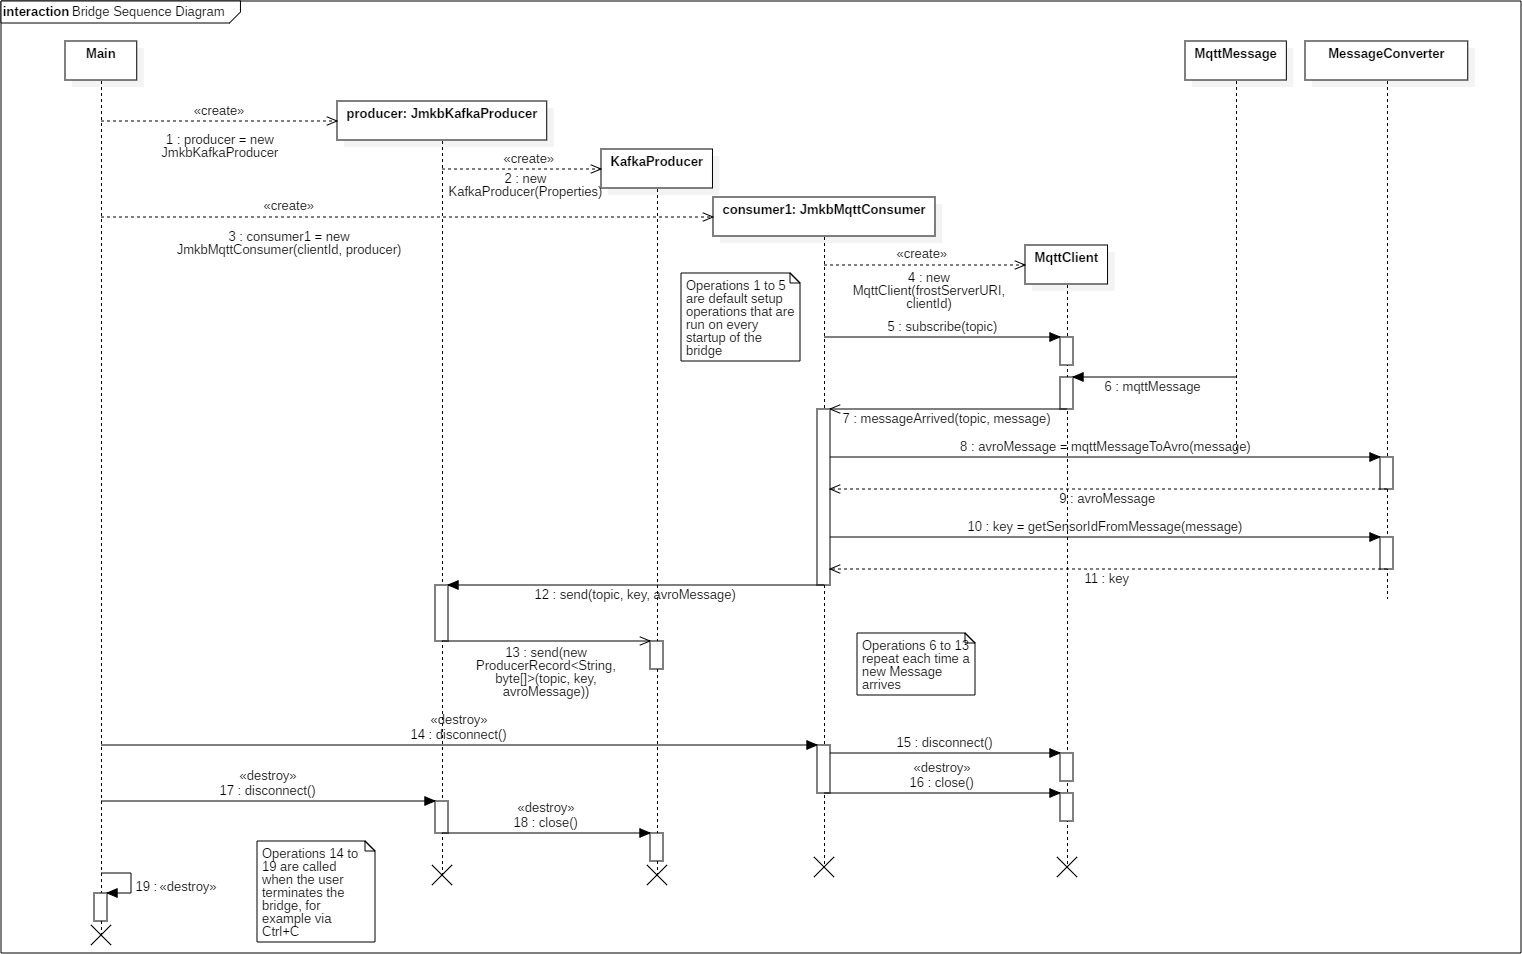
\includegraphics[width=\textheight,angle=90]{images/bridge/BridgeSequenceDiagram.png}
	\caption{Sequenzdiagramm Bridge}
\end{figure}
\newpage

\section{Core}
Beim Controller werden alle Topics welche von dem MQTT Producer generierten wurden subscribed (abonniert) in einer Schleife. Dann macht der Controller mit der generateOutputtopic einen neuen Output Topic für eine StreamProcessingStrategy, weil dieser einen Output Topic benötigt um die verarbeiteten Daten abzulagern.
Der Controller macht ein TopolgyBuilder Objekt, weil mit diesem die StreamProcessingStrategy, ausgeführt werden können. Der Controller übergibt mit addSource dem TopolgyBuilder einen Input Topic wo sich die zu verarbeiteten Daten in einem Kafka Stream enthalten sind. 
Der Controller macht eine neues StreamProcessingStrategy, welche die Methode ist wie die Inputdaten verarbeitet werden sollen. Der Controller übergibt den TopolgyBuilder mit addProcessor diese StreamProcessingStrategy.
Der Controller übergibt den TopolgyBuilder mit addSink den vorhin generieten Output Topic, welcher dieser als Daten Sink für von dem StreamProcessingStrategy verarbeiteten Daten nutzt. 
Der TopolgyBuilder startet dann mit kafkaStreamStart die StreamProcessingStrategy und dieser fängt mit apply aus dem Input Topic Daten in den Output Topic zu schreiben bis der TopolgyBuilder kafkaStreamclose aufruft und dann die Verarbeitung stoppt und der TopolgyBuilder und StreamProcessingStrategy zerstört werden.
\begin{figure}[!hbp]
	\centering
	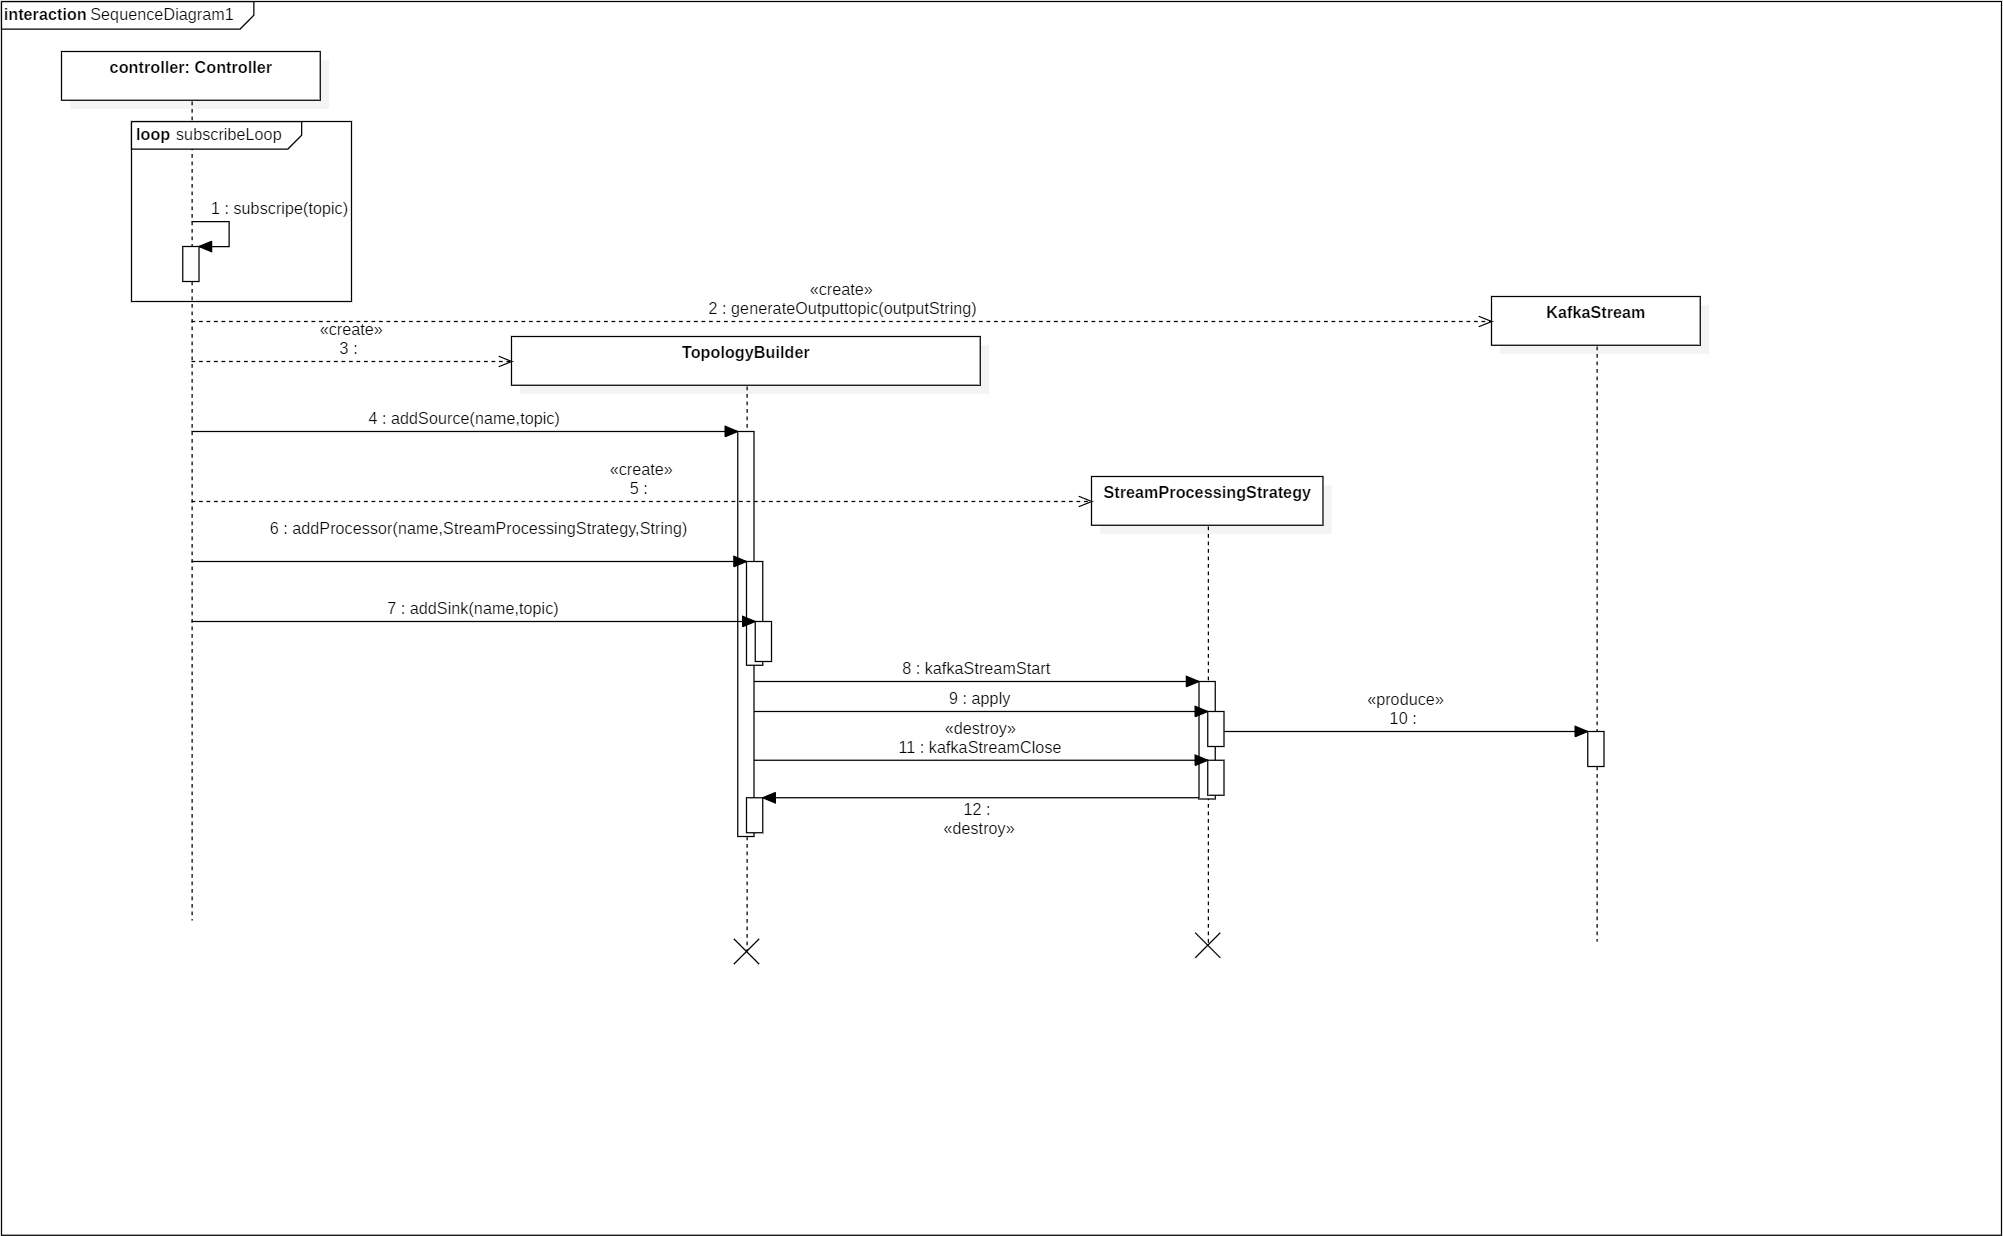
\includegraphics[width=\linewidth]{images/core/CoreSequenceDiagram.png}
	\caption{Sequenzdiagramm Core}
\end{figure}
\newpage

\section{Import}
Bei dem Import wird zuerst in dem Importordner nach Dateien gesucht und danach für jede vorhandene Datei ein separater Importprozess gestartet. Das folgende Sequenzdiagram stellt diesen Vorgang dar. Hier wird ausschließlich der Import behandelt, wer diesen Anstößt soll nicht Teil des Diagrams sein. \texttt{External} soll hier das Element darstellen, das den Import aufruft. Dazu wird ein \texttt{DataImporter} erstellt und seine Methode \texttt{startImportingFileData} aufgerufen, womit der Importvorgang startet.\\\\
Für jede Datei in dem Importordner wird nun ein \texttt{FrostSender} und einen \texttt{FilePath} der zum Pfad der Datei passt. Ist dies geschehen wird der \texttt{FileImporter} für diese Datei erschaffen und mit \texttt{addFileData} gestartet. Dazu wird der Pfad und der \texttt{FrostSender} mitübergeben. Aus dem Pfad wird jetzt eine \texttt{FileExtension} generiert, die dazu genutzt wird über den \texttt{ReaderType} eine Instanz einer Implementierung der \texttt{FileReaderStrategy} zu erhalten. Ist die \texttt{FileExtension} nicht bekannt würde es hier zu einer Exception kommen und der Import für diese Datei beendet.\\\\
In diesem Fall wurde als Beispiel eine \texttt{CSVReaderStrategy} genommen. Diese übernimmt den tatsächlichen Import der Daten aus der Datei zum FROST-Server vor. Dazu werden nach und nach einzelne Datensätze aus der Datei ausgelesen und über den \texttt{FrostSender} an den Server gesendet.
\begin{figure}[!hbp]
	\centering
	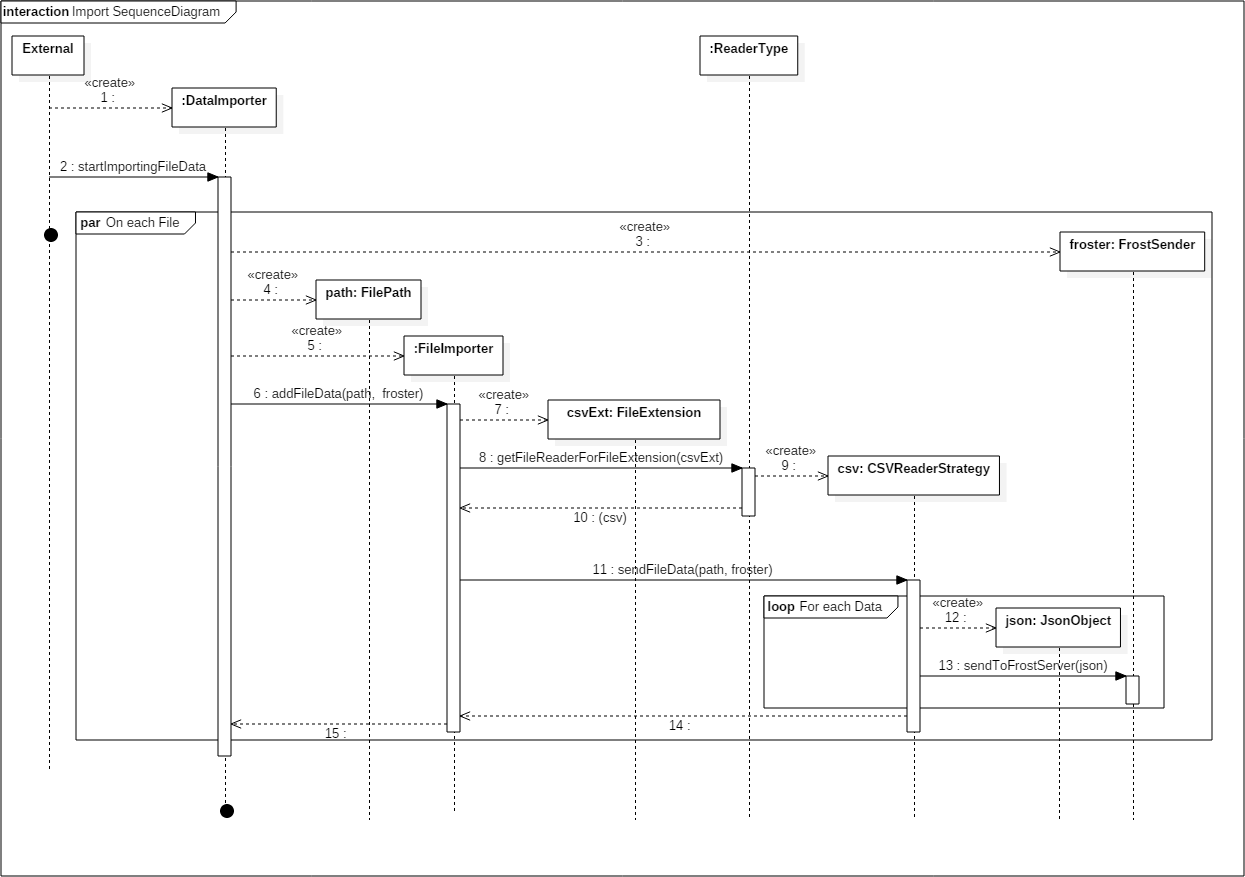
\includegraphics[width=0.9\linewidth]{images/import/ImportSequenceDiagram.png}
	\caption{Sequenzdiagramm Import}
\end{figure}
\newpage

\section{Graphite}
The user selects data to be requested through the use of the webinterface. Then the Servlet receives that request and tells us, what data we have to transfer. This information is passed on to the GraphDataTransferController, which in return passes it to a newly created KafkaToGraphiteConsumer. This also creates us a GraphiteSender automatically in the constructor. This KafkaToGraphiteConsumer is then run on the information. It gathers different properties that are needed for transfering data from Kafka from the GraphiteConfig and creates a KafkaConsumer to subscribe to Kafka. We then check whether we want to seek to the beginning . After that, we enter a loop. Here we start polling data from Kafka and storing them in a ConsumerRecords object. Finally, we check if there was any new information in the polled data. If there was, we send the data by using our GraphiteSender.
If we want to end the transferring of data, we have to call the wakeup method of our KafkaToGraphiteConsumer.
\begin{figure}[!hbp]
	\centering
	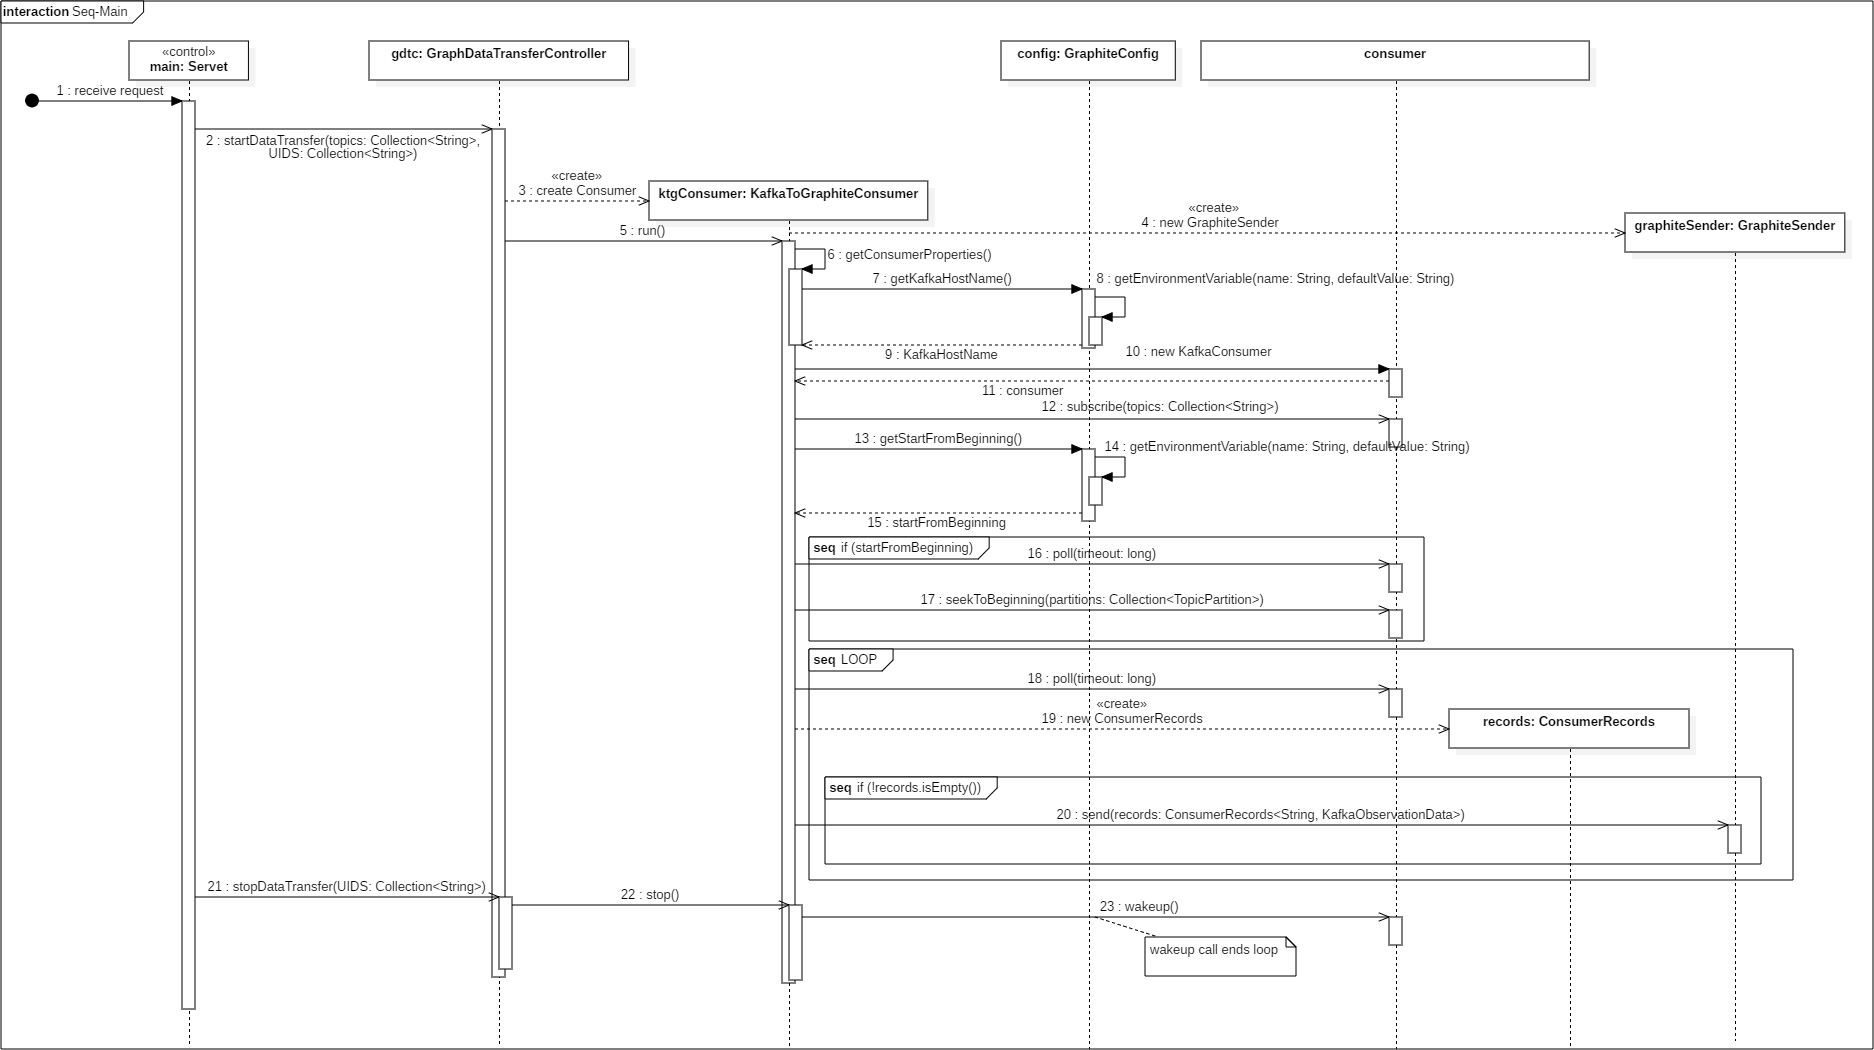
\includegraphics[width=\linewidth]{images/graphite/graphiteMainSequenceDiagram_small.png}
	\caption{Sequenzdiagramm Graphite}
\end{figure}
\newpage
Here the data that we want to send to Graphite is given to us directly. To do the job, the GraphiteSender gathers properties from the GraphiteConfig, that are needed for transferring data to Graphite. Afterwards, we start a loop. In this loop the GraphiteSender adds every observed property to the list of data to send to Graphite. The GraphiteSender does this by converting the data to metrics and then documenting the results. After adding all observed properties, we can finally sent the data to Graphite.
\begin{figure}[!hbp]
	\centering
	\includegraphics[width=\linewidth]{images/graphite/GraphiteSenderSequenceDiagram.png}
	\caption{Sequenzdiagramm GraphiteSender}
\end{figure}
\newpage

\section{Export}
Der Export wird in der WebGUI von einem Nutzer angefragt. Die Daten für diesen Export werden an das \texttt{ExportServlet} übertragen, das den tatsächlich export der Daten in eine Datei Verwaltet. Ist diese Datei einmal erstellt kann diese von dem Nutzer heruntergeladen werden. Dazu mehr im folgenden Abschnitt über den Download. Dieses Sequenzdiagram zeigt wie der Export der Daten in eine Datei durchgeführt wird.\\\\
Sobald ein Export angestoßen wird, startet das \texttt{ExportServlet} und die Methode \texttt{doGet} wird ausgeführt. Darin werden zuerst die \texttt{ExportProperties} ais der Datei ausgelesen und zu einem Objekt zusammengestellt, das unter anderem Eine \texttt{FileExtension} enthält. Danach wird ein \texttt{FileExporter} konstruiert, der in zwei Schritten vorgehen wird, um die Daten zu exportieren.\\\\
Im ersten Schritt, wird durch den Aufruf der \texttt{createFileInformation}-Methode der Export für den späteren Download eindeutig identifiziert indem ihm eine \texttt{DownloadID} zugewiesen wird. Ein \texttt{AlterableDownloadState} wird erstellt und dessen Methode \texttt{savePersistent} ausgeführt, damit die Information über den Download auch auf dem Server hinterlegt wird, sodass paralell zum Export auch eine Anfrage gesendet werden kann, ob die Datei bereits fertig für den Download ist. Die \texttt{DownloadID} wird dann an den Nutzer zurückgesendet sobald der zweite Teil mit der \texttt{createFile}-Methode des \texttt{FileExporters} gestartet wurde.\\\\
Im zweiten Teil findet dann der tatsächliche Export der Daten in eine Datei statt. Dazu wird zuerst ein \texttt{ExportStreamGenerator} konstruiert, dessen Methode \texttt{createExportStream} einen \texttt{KStream} der gewünschten Daten für den Export erzeugt. Die Gewünschten Daten gehen aus den \texttt{ExportProperties} hervor. Mit der \texttt{FileExtension} aus den \texttt{ExportProperties} kann jetzt ein \texttt{FileType} generiert werden, über dessen Methode \texttt{getFileWriter} eine neue Instanz einer Implementierung einer \texttt{FileWriterStrategy} zurückgegeben wird. Dazu wird die statische Methode \texttt{getFileWriterForFileExtension} der Utilityklasse \texttt{FileTypesUtility} verwendet. In diesem Sequenzdiagram wird als Beispiel eine Instanz der \texttt{CSVWriterStrategy} verwendet.\\\\
Nun wird ein passender neuer Pfad als \texttt{FilePath} erzeugt, um die Datei zu erzeugen. Dazu wird die Methode \texttt{saveToFile} eines \texttt{FileWriterStrategy} genutzt. In diesem Fall einer \texttt{CSVWriterStrategy}. Diese Methode benötigt den ZielPfad und den Stream der Daten und erzeugt daraus eine Datei. Ist dies beendet, wird der \texttt{AlterableDownloadState} dazu genutzt die nötigen Informationen abzuspeichern. Zuerst wird der Pfad der Datei eingegeben und anschließend, dass die Datei bereit für den Download ist. Zum Schluß wird noch mit \texttt{savePersistent} sichergestellt, dass andere Instanzen eines \texttt{DownloadState} diese Information abrufen können.
\begin{figure}[!hbp]
	\centering
	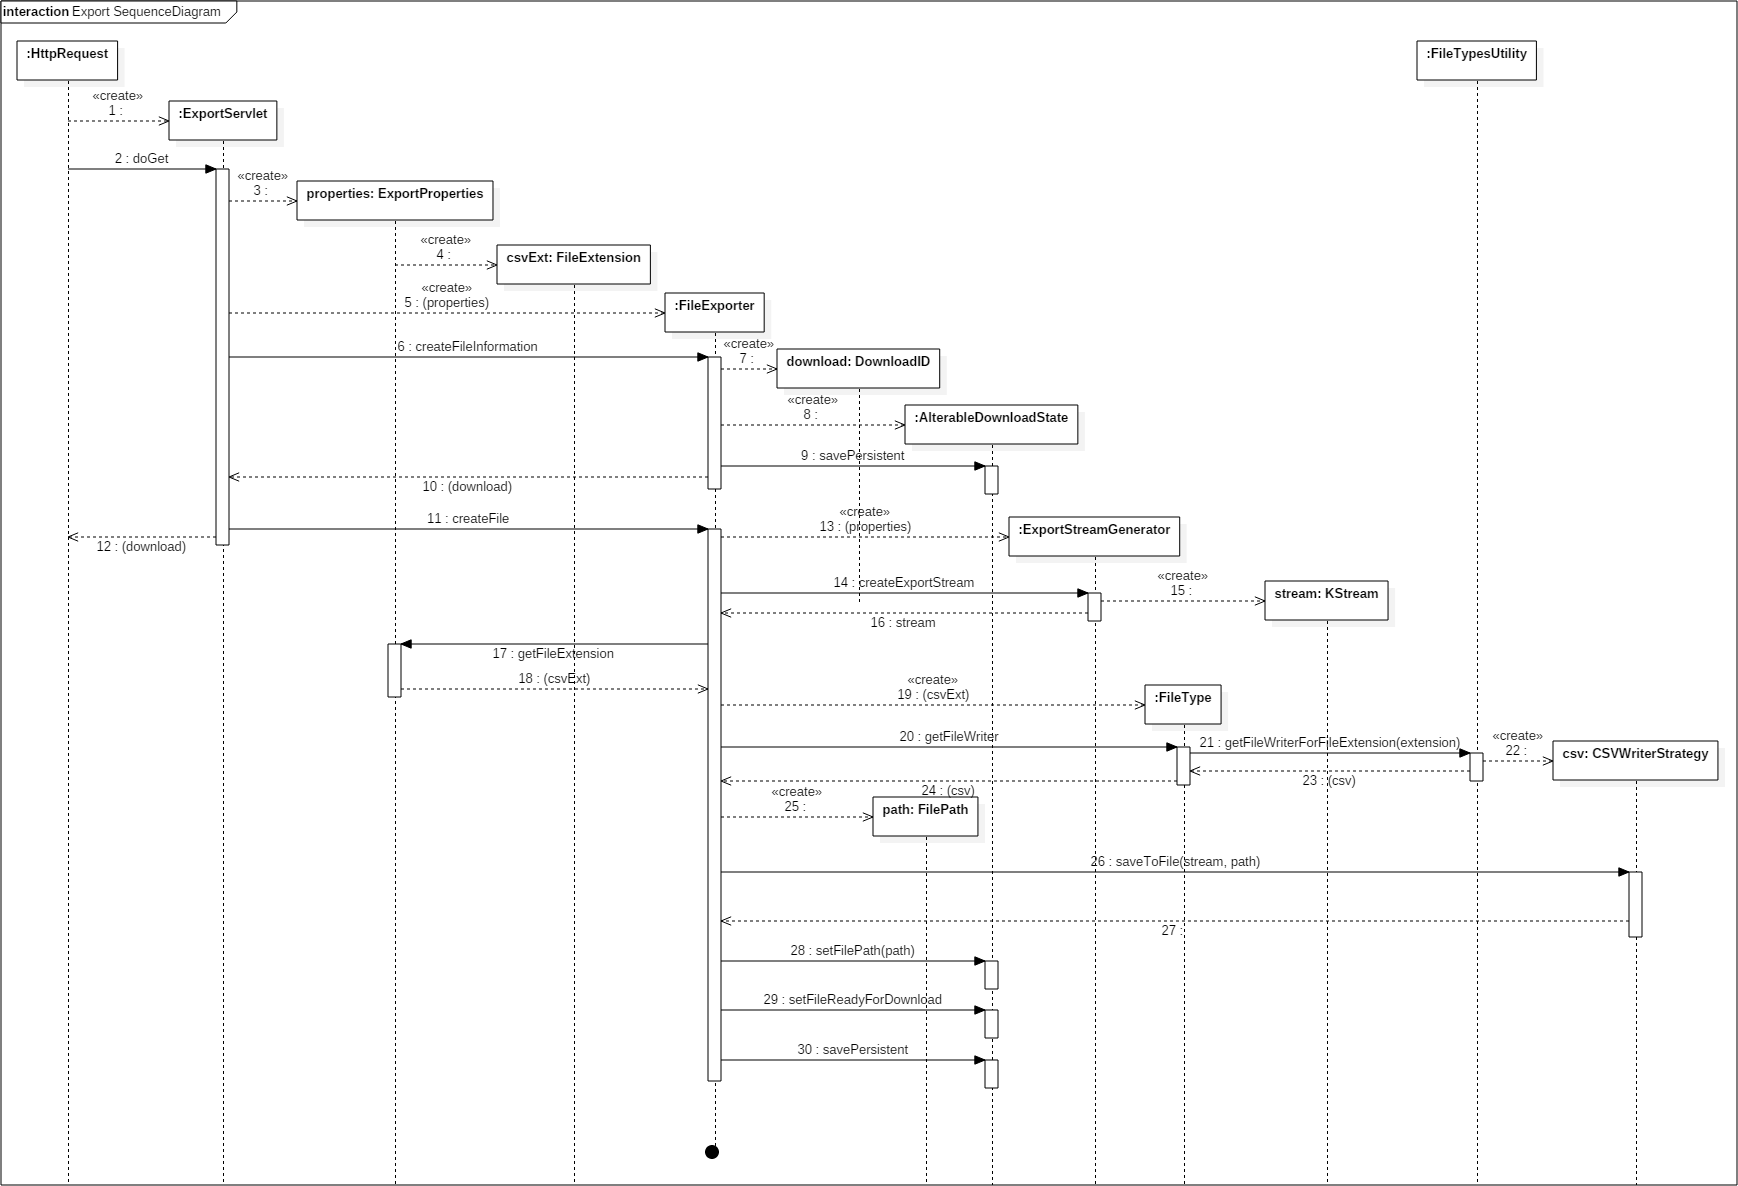
\includegraphics[width=1.25\linewidth,angle=90]{images/export/ExportSequenceDiagram.png}
	\caption{Sequenzdiagramm Export}
\end{figure}
\newpage
Ein Download wird grundsätzlich von einem Nutzer aus einem Browserfenster angefragt. Dazu wird das \texttt{DownloadServlet} benutzt. Diese wird vom Server erstellt sobald eine Anfrage des Nutzer einkommt. Dann wird \texttt{doGet} aufgerufen und das Servlet beginnt mit seiner Aufgabe, die in diesem Sequenzdiagram dargestellt wird.\\\\
Die Anfrage des nutzers enthält eine DownloadID, die für eine bestimmte Datei auf dem Server steht. Diese wird benutzt um eine \texttt{DownloadID} Objekt zu erstellen, das dazu dient einen \texttt{DownloadState} zu konstruieren. Dieser holt sich, sobald er erstellt wurde, die Informationen zu dem betreffenden Download. Diese Informationen könnten in einer Datei liegen. Nun wird zuerst geprüft, ob die Datei bereit für den Download ist, dazu dient die Methode \texttt{isFileReadyForDownload}. Ist dies der Fall kann nun mit der \texttt{getFilePath}-Methode nach dem Pfad der Datei gefragt werden. Dieser wird nun vom \texttt{DownloadServlet} genutzt, um die Datei dem Nutzer zu schicken.\\\\
Der Vorgang bei dem \texttt{StatusServlet} ist sehr Ähnlich. Dort geht es darum in Erfahrung zu bringen, ob eine Download bereit ist, um zum Beispiel zu wissen, ob dem Nutzer bereits ein Download-Button gezeigt werden kann. Der einzige Unterschied liegt darin, dass dort nicht nach dem Pfad gesucht wird, sobndern gleich das Ergebnis der \texttt{isFileReadyForDownload} zurückgeschickt wird. Aus diesem Grund wurde darauf verzichtet ein separates Sequenzdiagram dafür zu erstellen.
\begin{figure}[!hbp]
	\centering
	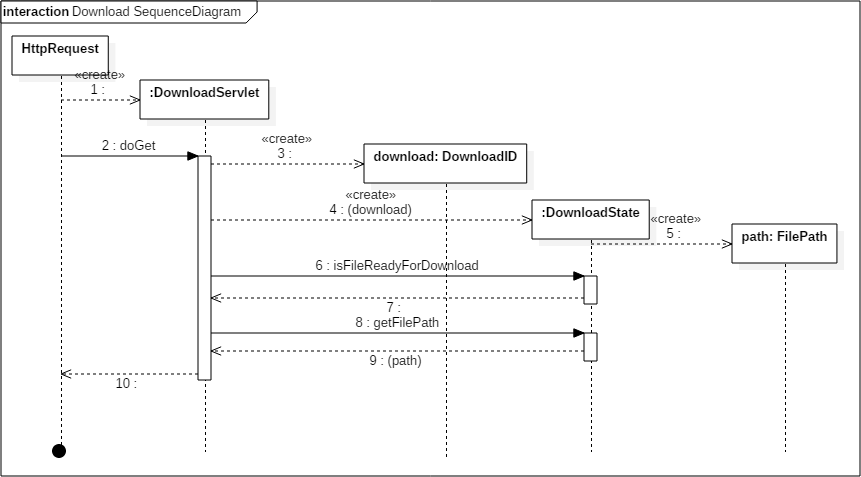
\includegraphics[width=\linewidth]{images/export/DownloadSequenceDiagram.png}
	\caption{Sequenzdiagramm Download}
\end{figure}
